%% bare_conf.tex
%% V1.4b
%% 2015/08/26
%% by Michael Shell
%% See:
%% http://www.michaelshell.org/
%% for current contact information.
%%
%% This is a skeleton file demonstrating the use of IEEEtran.cls
%% (requires IEEEtran.cls version 1.8b or later) with an IEEE
%% conference paper.
%%
%% Support sites:
%% http://www.michaelshell.org/tex/ieeetran/
%% http://www.ctan.org/pkg/ieeetran
%% and
%% http://www.ieee.org/

%%*************************************************************************
%% Legal Notice:
%% This code is offered as-is without any warranty either expressed or
%% implied; without even the implied warranty of MERCHANTABILITY or
%% FITNESS FOR A PARTICULAR PURPOSE! 
%% User assumes all risk.
%% In no event shall the IEEE or any contributor to this code be liable for
%% any damages or losses, including, but not limited to, incidental,
%% consequential, or any other damages, resulting from the use or misuse
%% of any information contained here.
%%
%% All comments are the opinions of their respective authors and are not
%% necessarily endorsed by the IEEE.
%%
%% This work is distributed under the LaTeX Project Public License (LPPL)
%% ( http://www.latex-project.org/ ) version 1.3, and may be freely used,
%% distributed and modified. A copy of the LPPL, version 1.3, is included
%% in the base LaTeX documentation of all distributions of LaTeX released
%% 2003/12/01 or later.
%% Retain all contribution notices and credits.
%% ** Modified files should be clearly indicated as such, including  **
%% ** renaming them and changing author support contact information. **
%%*************************************************************************


% *** Authors should verify (and, if needed, correct) their LaTeX system  ***
% *** with the testflow diagnostic prior to trusting their LaTeX platform ***
% *** with production work. The IEEE's font choices and paper sizes can   ***
% *** trigger bugs that do not appear when using other class files.       ***                          ***
% The testflow support page is at:
% http://www.michaelshell.org/tex/testflow/



\documentclass[conference]{IEEEtran}
% Some Computer Society conferences also require the compsoc mode option,
% but others use the standard conference format.
%
% If IEEEtran.cls has not been installed into the LaTeX system files,
% manually specify the path to it like:
% \documentclass[conference]{../sty/IEEEtran}





% Some very useful LaTeX packages include:
% (uncomment the ones you want to load)


% *** MISC UTILITY PACKAGES ***
%
%\usepackage{ifpdf}
% Heiko Oberdiek's ifpdf.sty is very useful if you need conditional
% compilation based on whether the output is pdf or dvi.
% usage:
% \ifpdf
%   % pdf code
% \else
%   % dvi code
% \fi
% The latest version of ifpdf.sty can be obtained from:
% http://www.ctan.org/pkg/ifpdf
% Also, note that IEEEtran.cls V1.7 and later provides a builtin
% \ifCLASSINFOpdf conditional that works the same way.
% When switching from latex to pdflatex and vice-versa, the compiler may
% have to be run twice to clear warning/error messages.






% *** CITATION PACKAGES ***
%
%\usepackage{cite}
% cite.sty was written by Donald Arseneau
% V1.6 and later of IEEEtran pre-defines the format of the cite.sty package
% \cite{} output to follow that of the IEEE. Loading the cite package will
% result in citation numbers being automatically sorted and properly
% "compressed/ranged". e.g., [1], [9], [2], [7], [5], [6] without using
% cite.sty will become [1], [2], [5]--[7], [9] using cite.sty. cite.sty's
% \cite will automatically add leading space, if needed. Use cite.sty's
% noadjust option (cite.sty V3.8 and later) if you want to turn this off
% such as if a citation ever needs to be enclosed in parenthesis.
% cite.sty is already installed on most LaTeX systems. Be sure and use
% version 5.0 (2009-03-20) and later if using hyperref.sty.
% The latest version can be obtained at:
% http://www.ctan.org/pkg/cite
% The documentation is contained in the cite.sty file itself.






% *** GRAPHICS RELATED PACKAGES ***
%
\ifCLASSINFOpdf
  \usepackage[pdftex]{graphicx}
  % declare the path(s) where your graphic files are
  \graphicspath{{Figures}{../jpeg/}}
  % and their extensions so you won't have to specify these with
  % every instance of \includegraphics
  \DeclareGraphicsExtensions{.pdf,.jpeg,.png}
\else
  % or other class option (dvipsone, dvipdf, if not using dvips). graphicx
  % will default to the driver specified in the system graphics.cfg if no
  % driver is specified.
  % \usepackage[dvips]{graphicx}
  % declare the path(s) where your graphic files are
  % \graphicspath{{../eps/}}
  % and their extensions so you won't have to specify these with
  % every instance of \includegraphics
  % \DeclareGraphicsExtensions{.eps}
\fi
% graphicx was written by David Carlisle and Sebastian Rahtz. It is
% required if you want graphics, photos, etc. graphicx.sty is already
% installed on most LaTeX systems. The latest version and documentation
% can be obtained at: 
% http://www.ctan.org/pkg/graphicx
% Another good source of documentation is "Using Imported Graphics in
% LaTeX2e" by Keith Reckdahl which can be found at:
% http://www.ctan.org/pkg/epslatex
%
% latex, and pdflatex in dvi mode, support graphics in encapsulated
% postscript (.eps) format. pdflatex in pdf mode supports graphics
% in .pdf, .jpeg, .png and .mps (metapost) formats. Users should ensure
% that all non-photo figures use a vector format (.eps, .pdf, .mps) and
% not a bitmapped formats (.jpeg, .png). The IEEE frowns on bitmapped formats
% which can result in "jaggedy"/blurry rendering of lines and letters as
% well as large increases in file sizes.
%
% You can find documentation about the pdfTeX application at:
% http://www.tug.org/applications/pdftex





% *** MATH PACKAGES ***
%
%\usepackage{amsmath}
% A popular package from the American Mathematical Society that provides
% many useful and powerful commands for dealing with mathematics.
%
% Note that the amsmath package sets \interdisplaylinepenalty to 10000
% thus preventing page breaks from occurring within multiline equations. Use:
%\interdisplaylinepenalty=2500
% after loading amsmath to restore such page breaks as IEEEtran.cls normally
% does. amsmath.sty is already installed on most LaTeX systems. The latest
% version and documentation can be obtained at:
% http://www.ctan.org/pkg/amsmath





% *** SPECIALIZED LIST PACKAGES ***
%
%\usepackage{algorithmic}
% algorithmic.sty was written by Peter Williams and Rogerio Brito.
% This package provides an algorithmic environment fo describing algorithms.
% You can use the algorithmic environment in-text or within a figure
% environment to provide for a floating algorithm. Do NOT use the algorithm
% floating environment provided by algorithm.sty (by the same authors) or
% algorithm2e.sty (by Christophe Fiorio) as the IEEE does not use dedicated
% algorithm float types and packages that provide these will not provide
% correct IEEE style captions. The latest version and documentation of
% algorithmic.sty can be obtained at:
% http://www.ctan.org/pkg/algorithms
% Also of interest may be the (relatively newer and more customizable)
% algorithmicx.sty package by Szasz Janos:
% http://www.ctan.org/pkg/algorithmicx




% *** ALIGNMENT PACKAGES ***
%
\usepackage{array}
% Frank Mittelbach's and David Carlisle's array.sty patches and improves
% the standard LaTeX2e array and tabular environments to provide better
% appearance and additional user controls. As the default LaTeX2e table
% generation code is lacking to the point of almost being broken with
% respect to the quality of the end results, all users are strongly
% advised to use an enhanced (at the very least that provided by array.sty)
% set of table tools. array.sty is already installed on most systems. The
% latest version and documentation can be obtained at:
% http://www.ctan.org/pkg/array


% IEEEtran contains the IEEEeqnarray family of commands that can be used to
% generate multiline equations as well as matrices, tables, etc., of high
% quality.




% *** SUBFIGURE PACKAGES ***
%\ifCLASSOPTIONcompsoc
%  \usepackage[caption=false,font=normalsize,labelfont=sf,textfont=sf]{subfig}
%\else
%  \usepackage[caption=false,font=footnotesize]{subfig}
%\fi
% subfig.sty, written by Steven Douglas Cochran, is the modern replacement
% for subfigure.sty, the latter of which is no longer maintained and is
% incompatible with some LaTeX packages including fixltx2e. However,
% subfig.sty requires and automatically loads Axel Sommerfeldt's caption.sty
% which will override IEEEtran.cls' handling of captions and this will result
% in non-IEEE style figure/table captions. To prevent this problem, be sure
% and invoke subfig.sty's "caption=false" package option (available since
% subfig.sty version 1.3, 2005/06/28) as this is will preserve IEEEtran.cls
% handling of captions.
% Note that the Computer Society format requires a larger sans serif font
% than the serif footnote size font used in traditional IEEE formatting
% and thus the need to invoke different subfig.sty package options depending
% on whether compsoc mode has been enabled.
%
% The latest version and documentation of subfig.sty can be obtained at:
% http://www.ctan.org/pkg/subfig




% *** FLOAT PACKAGES ***
%
%\usepackage{fixltx2e}
% fixltx2e, the successor to the earlier fix2col.sty, was written by
% Frank Mittelbach and David Carlisle. This package corrects a few problems
% in the LaTeX2e kernel, the most notable of which is that in current
% LaTeX2e releases, the ordering of single and double column floats is not
% guaranteed to be preserved. Thus, an unpatched LaTeX2e can allow a
% single column figure to be placed prior to an earlier double column
% figure.
% Be aware that LaTeX2e kernels dated 2015 and later have fixltx2e.sty's
% corrections already built into the system in which case a warning will
% be issued if an attempt is made to load fixltx2e.sty as it is no longer
% needed.
% The latest version and documentation can be found at:
% http://www.ctan.org/pkg/fixltx2e


%\usepackage{stfloats}
% stfloats.sty was written by Sigitas Tolusis. This package gives LaTeX2e
% the ability to do double column floats at the bottom of the page as well
% as the top. (e.g., "\begin{figure*}[!b]" is not normally possible in
% LaTeX2e). It also provides a command:
%\fnbelowfloat
% to enable the placement of footnotes below bottom floats (the standard
% LaTeX2e kernel puts them above bottom floats). This is an invasive package
% which rewrites many portions of the LaTeX2e float routines. It may not work
% with other packages that modify the LaTeX2e float routines. The latest
% version and documentation can be obtained at:
% http://www.ctan.org/pkg/stfloats
% Do not use the stfloats baselinefloat ability as the IEEE does not allow
% \baselineskip to stretch. Authors submitting work to the IEEE should note
% that the IEEE rarely uses double column equations and that authors should try
% to avoid such use. Do not be tempted to use the cuted.sty or midfloat.sty
% packages (also by Sigitas Tolusis) as the IEEE does not format its papers in
% such ways.
% Do not attempt to use stfloats with fixltx2e as they are incompatible.
% Instead, use Morten Hogholm'a dblfloatfix which combines the features
% of both fixltx2e and stfloats:
%
% \usepackage{dblfloatfix}
% The latest version can be found at:
% http://www.ctan.org/pkg/dblfloatfix




% *** PDF, URL AND HYPERLINK PACKAGES ***
%
%\usepackage{url}
% url.sty was written by Donald Arseneau. It provides better support for
% handling and breaking URLs. url.sty is already installed on most LaTeX
% systems. The latest version and documentation can be obtained at:
% http://www.ctan.org/pkg/url
% Basically, \url{my_url_here}.




% *** Do not adjust lengths that control margins, column widths, etc. ***
% *** Do not use packages that alter fonts (such as pslatex).         ***
% There should be no need to do such things with IEEEtran.cls V1.6 and later.
% (Unless specifically asked to do so by the journal or conference you plan
% to submit to, of course. )


% correct bad hyphenation here
\hyphenation{op-tical net-works semi-conduc-tor}

\usepackage{multirow}

\usepackage{tikz-timing}[2009/05/15]
%\usepackage{tikz}
%\tikzset{every picture/.style={line width=0.75pt}} %set default line width to 0.75pt        

\newcolumntype{P}[1]{>{\centering\arraybackslash}p{#1}}
\newcolumntype{L}[1]{>{\arraybackslash}p{#1}}

\begin{document}
%
% paper title
% Titles are generally capitalized except for words such as a, an, and, as,
% at, but, by, for, in, nor, of, on, or, the, to and up, which are usually
% not capitalized unless they are the first or last word of the title.
% Linebreaks \\ can be used within to get better formatting as desired.
% Do not put math or special symbols in the title.
\title{FPGA-based Sliding Windowed Infinite Fourier Transform for Doppler frequency estimation}

% author names and affiliations
% use a multiple column layout for up to three different
% affiliations
\author{\IEEEauthorblockN{Prashant Dabholkar, Christopher Gilliam}
\IEEEauthorblockA{School of Engineering\\
RMIT University\\
Melbourne, Australia\\
Email: \{prashant.dabholkar,christopher.gilliam\}@rmit.edu.au}
}

% conference papers do not typically use \thanks and this command
% is locked out in conference mode. If really needed, such as for
% the acknowledgment of grants, issue a \IEEEoverridecommandlockouts
% after \documentclass

% for over three affiliations, or if they all won't fit within the width
% of the page, use this alternative format:
% 
%\author{\IEEEauthorblockN{Michael Shell\IEEEauthorrefmark{1},
%Homer Simpson\IEEEauthorrefmark{2},
%James Kirk\IEEEauthorrefmark{3}, 
%Montgomery Scott\IEEEauthorrefmark{3} and
%Eldon Tyrell\IEEEauthorrefmark{4}}
%\IEEEauthorblockA{\IEEEauthorrefmark{1}School of Electrical and Computer Engineering\\
%Georgia Institute of Technology,
%Atlanta, Georgia 30332--0250\\ Email: see http://www.michaelshell.org/contact.html}
%\IEEEauthorblockA{\IEEEauthorrefmark{2}Twentieth Century Fox, Springfield, USA\\
%Email: homer@thesimpsons.com}
%\IEEEauthorblockA{\IEEEauthorrefmark{3}Starfleet Academy, San Francisco, California 96678-2391\\
%Telephone: (800) 555--1212, Fax: (888) 555--1212}
%\IEEEauthorblockA{\IEEEauthorrefmark{4}Tyrell Inc., 123 Replicant Street, Los Angeles, California 90210--4321}}


% use for special paper notices
%\IEEEspecialpapernotice{(Invited Paper)}


% make the title area
\maketitle

% As a general rule, do not put math, special symbols or citations
% in the abstract
\begin{abstract}
This is the abstract

\end{abstract}

% no keywords

% For peer review papers, you can put extra information on the cover
% page as needed:
% \ifCLASSOPTIONpeerreview
% \begin{center} \bfseries EDICS Category: 3-BBND \end{center}
% \fi
%
% For peerreview papers, this IEEEtran command inserts a page break and
% creates the second title. It will be ignored for other modes.
\IEEEpeerreviewmaketitle


\section{Introduction}
\label{Sec:Introduction}

Position and speed detection system used in the automotive, security and surveillance sector typically use a Continuous Wave (CW) or Frequency Modulated Continuous Wave (FMCW) Radar. In these systems, the baseband processors analyse the Doppler information in the spectrum of the received signal to accurately estimate speed and position of the target. Discrete Fourier Transform is an important tool required to perform spectral analysis of the data that has a time varying component in its frequency. One of the most common methods of computing the DFT of a signal is using the Fast Fourier transform (FFT). FFT accelerators available on Digital Signal Processors, use a pipelined architecture to compute the FFT. These pipelined architectures are especially suitable for this purpose since they provide high throughput and low power, as well as low latency\cite{Mookherjee2015}. In addition to the pipelining, in systems where high throughput is a critical requirement, several samples of an input signal may be processed in parallel leading to the development of the 2-parallel Radix-2 \cite{Ayinala2012} and 8-parallel Radix-2 \cite{Mookherjee2015} algorithms. 

However for position and speed detection systems that have to work in real time, the frequency difference between a transmitted signal and its received reflection is used to detect the target range and velocity. The return signal, which has a different frequency, is called a ‘beat-signal’. Depending on the speed of the moving target, the bandwidth of the received beat-signal decreases by a few kiloHertz regardless of the transmitted bandwidth, the complexity of the signal processing can be reduced, compared with that of conventional spectrum analysis.and are concerned only with a small time-varying subset of the frequency spectrum around the beat frequency, the DFT needs to be calculated almost every sample. In such a scenario, the FFT computation scheme is not the best solution because it iig essentially a batch process and computing the $N$-point FFT requires the system to wait for $N$ time samples. 

The sliding window DFT (SDFT) is a popular alternative algorithm that was introduced by Springer \cite{Springer1988} and later improved by Jacobsen et al. \cite{Jacobsen2003}. The algorithm is efficient however, it is limited in that it is only marginally stable and requires storing $N$
previous samples. Grado et al. \cite{Grado2017} introduced the idea of a Sliding Windowed Infinite Fourier Transform (SWIFT) that has several advantages over the SDFT. The proposed algorithm is guaranteed stable and has an improved frequency domain sampling. In addition, unlike the SDFT that uses a rectangular window, the SWIFT uses an exponentially decaying window that assigns greater weights to recent samples. 

In recent years, frequency-modulated continuous-wave (FMCW) radars have been used in vehicle applications. In FMCW radars, linear ramps are generated and transmitted. The frequency difference between a transmitted signal and its received reflection is used to detect the target range and velocity. The return signal, which has a different frequency, is called a ‘beat-signal’. Because the bandwidth of the received beat-signal decreases by less than a dozen MHz regardless of the transmitted bandwidth, the complexity of the signal processing can be reduced, compared with that of conventional spectrum analysis.
\section{SWIFT Algorithm}
\label{Sec:SWIFT}

The Sliding Windowed Infinite Foutier Transform (SWIFT) is a type of sliding DTFT proposed by Grado et al. \cite{Grado2017} that uses an infinite-length causal exponential function. A detailed discussion of the function, it derivation and equivalence to the windowed DTFT is available in \cite{Grado2017}. Here, we review some of the ideas and equations that are essential to understanding the FPGA implementation that follows. The exponential windowing function in the SWIFT is given by  
\begin{equation}
w[m] = \begin{cases}e^{m/\tau} & m \leq 0\\0 & m > 0\end{cases},
\end{equation}

where $w[m]$ is the window function that is applied to the discrete samples of the signal, $m = 0$ is the current sample and $\tau$ is the time constant. The exponential window function gives greater weight to more recent samples. A smaller value of $\tau$ makes the SWIFT extremely sensitive to transient changes in signal power, while a larger value of $\tau$ results in a Fourier Transform that responds much slower to instantaneous changes in the signal power. The DTFT is given by the following expression

\begin{equation}
\label{eq:x_n}
X_n(\omega) = \sum_{m=-\infty}^0 e^{m/\tau} x[n+m] e^{-j\omega m},
\end{equation}

where $\omega$ ($ = 2\pi f/f_s$)is continuous in the frequency domain and has normalized units of radians/sample. For an FPGA implementation it is necessary to simplify Equation \ref{eq:x_n} into a recursive formula relating the previous $X_{n-1}(\omega)$ value to the $X_n(\omega)$ value of interest. Substituting $(n-1)$ and $n$ in Equation \ref{eq:x_n} gives the following simplified relation

\begin{equation}
\label{eq:X_n_X_n1}
X_n(\omega) = e^{-1/\tau}e^{j\omega}X_{n-1}(\omega) + x[n].
\end{equation}

It can be seen that unlike the SDFT, The  SWIFT  algorithm  calculates $X_n$ by phase shifting and decaying the previous $X_{n-1}$ and adding the  current $x[n]$ sample. The SWIFT requires only one complex multiply and one real add per sample per bin. Figure \ref{fig:SWIFT_structure} shows an implementation of the SWIFT algorithm as an IIR filter with a complex resonator.

\begin{figure}
\centering
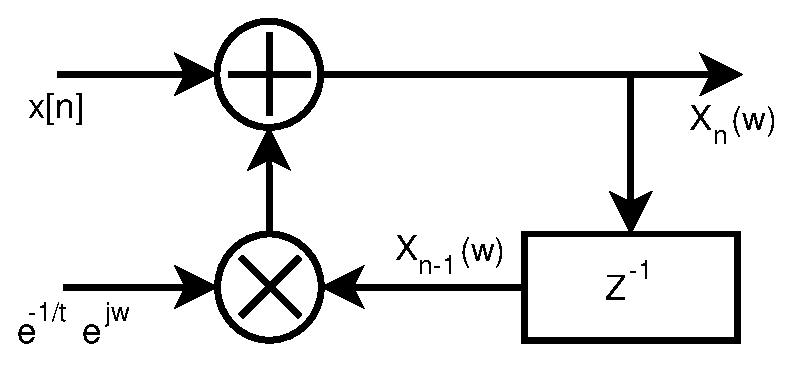
\includegraphics[width=0.75\columnwidth]{Figures/fig_SWIFT_algorithm.eps}
\caption{Structure of a SWIFT algorithm unit to compute the energy in a single frequency bin}
\label{fig:SWIFT_structure}
\end{figure}

It may be noted that while the Windowed Sliding Window DFT is a Discrete Fourier Transform, the SWIFT is continuous in the frequency domain. With $N$ samples in the window, an SDFT will have a normalized frequency resolution of $2\pi/N$. To achieve a finer resolution, an SDFT implementation would have to increase the value of $N$, i.e. the number of samples in the sliding window. This in turn requires additional storage and also reduces the temporal resolution of the DFT. 
In a SWIFT implementation however, a finer frequency resolution doesn't require one to include more samples in the computation. This is an important characteristic of the SWIFT because, for applications where only a subset of the complete frequency spectrum is of interest, it is advantageous to have an algorithm that can increase the frequency resolution without having to increase the digital sample storage. 
\section{Proposed FPGA implementation of SWIFT}
\label{Sec:FPGA}

In this section we describe the proposed FPGA implementation of the SWIFT algorithm as described by Equation \ref{eq:X_n_X_n1}. As seen in Figure \ref{fig:SWIFT_structure}, the fundamental computation unit hereafter referred to as a `SWIFT slice' consists of a complex multiplier, a complex adder and a single delay element. When implementing this function inside a FPGA, a sample $x(n)$  needs to pass through the multiplier and be available at the input of the adder when the next sample $x(n+1)$ comes in. On an FPGA, the complex multiplier and complex adder are implemented using the floating point add (FPADD) and floating point multiply (FPMUL) library functions available in the FPGA design tool. The complex floating point adder requires two FPADD operators, while the complex floating point multiplier requires four FPMUL and two FPADD operators. Thus a single `SWIFT slice' requires a total of 4 floating point adders and 4 floating point multipliers. The organization of the library functions to achieve the functionality of the `SWIFT slice' is shown in Figure \ref{fig:SWIFT_unit}.

\begin{figure}[tbp]
\centering
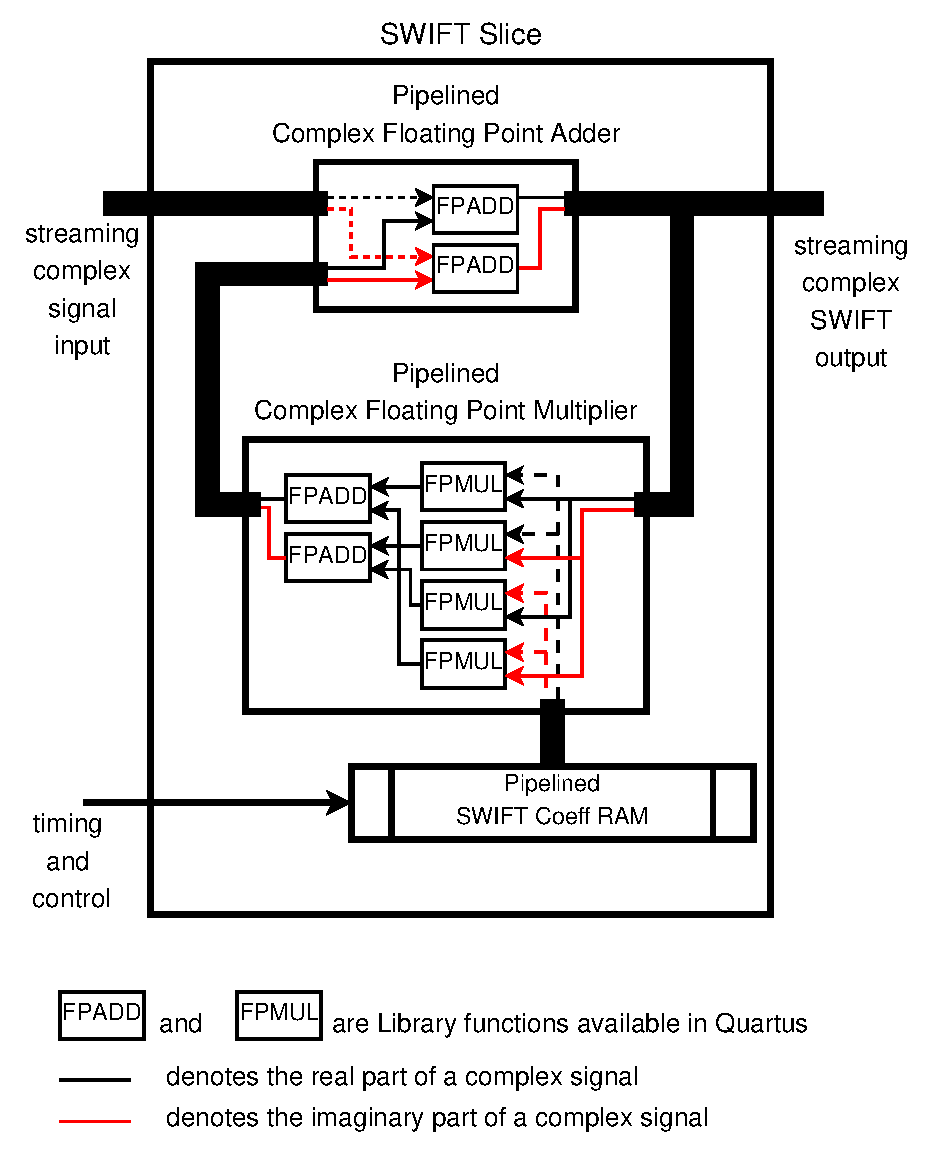
\includegraphics[width=0.85\columnwidth]{Figures/fig_SWIFT_slice.eps}
\caption{Block diagram of SWIFT slice}
\label{fig:SWIFT_unit}
\end{figure}

An important characteristic of the hardware library functions FPADD and FPMUL is their latency measured in terms of the number of clock cycles required to produce a valid output after the inputs are stable. These latencies are non-zero and this implies that a sample $x[n-1]$ presented at the input of the `SWIFT unit' will take some finite number of clock cycles to pass through all the modules and generate a value for $e^{-1/\tau}e^{j\omega}X_{n-1}(\omega)$ that can be added to the next sample $x[n]$.

If the the adder and the multiplier have latencies of $cyc_{fa}$ $cyc_{fm}$, and the data samples are presented at the input at a rate of $Srate_{din}$ Msps, the minimum frequency of the clock $f_{SWIFT}$ in MHz required to run the SWIFT slice is given by
\begin{equation}
\label{eq:swift_freq}
f_{SWIFT} \geq (cyc_{fa} + cyc_{fm} + cyc_{fa}) \times srate_{din} 
\end{equation}. 

Equation \ref{eq:swift_freq} implies that SWIFT slice needs to run at a higher frequency than the sampling frequency of the incoming signal. The higher frequency of the SWIFT clock ensures that a data sample being processed by the SWIFT algorithm, passes through the complex adder and multiplier and is available back at the input of the complex adder before the next sample comes in. Figure \ref{fig:SWIFT_slice_waveform} illustrates the timing relation between the signals inside a SWIFT unit. An interesting consequence of this relation is that when the left and right sides in Equation \ref{eq:swift_freq} are equal, a separate storage element to delay the computed value of $X_n(\omega)$ is not required, as the delay through the computation units achieves this functionality.

\begin{figure*}
\centering
\begin{tikztimingtable}
  	sample clock  & 9.5L 3{9.5C} 9.5L \\
  	SWIFT clock   & 95{0.5C}\\
  	sample  	  & [timing/text format={\large}]9.5D{x[n-1]} N(S1) {} 19D{x[n]} {} 19D{x[n+1]}\\
 	\textbf{Adder} \\
  	FPADD out  	  & [timing/text format={\large}]16.5D{$X_{n-1}(\omega_x)$} N(S2) {} N(FA1) 19D{$X_n(\omega_x)$} {} 12D{$X_{n+1}(\omega_x)$} \\
    \textbf{SWIFT RAM} \\
   	SWIFT Coeff	  & [timing/text format={\large}]47.5D{($\tau_x, \omega_x)$} \\
    \textbf{Mutliplier} \\
   	FPMUL out  	  & [timing/text format={\large}]21.5D{$Dmul_{n-1}(\omega_x)$} {} N(FM1) 19D{$Dmul_n(\omega_x)$} {} 7D{} \\
    FPADD out  	  & [timing/text format={\large}]28.5D{$Dadd_{n-1}(\omega_x)$} {} N(FA2) 19D{$Daddr_n(\omega_x)$} {} D{} \\ \\ 	
	\extracode
  	\tablerules
	\begin{pgfonlayer}{background}
    	\vertlines [help lines] {9.5,16.5,21.5,28.5};
        
        \node [anchor = mid ] at (13,-5){\small $cyc_{fa}$};
        \draw [<->] (9.5,-6) -- (16.5,-6);
        
        \node [anchor = mid ] at (19,-13){\small $cyc_{fm}$};
        \draw [<->] (16.5,-14) -- (21.5,-14);
        
        \node [anchor = mid] at (25,-19){\small $cyc_{fa}$};
        \draw [<->] (21.5,-20) -- (28.5,-20);
  	\end{pgfonlayer}
\end{tikztimingtable}
\caption{SWIFT slice timing waveform for a frequency $\omega_x$}
\label{fig:SWIFT_slice_waveform}
\end{figure*}


In a FFT computation the frequency resolution is a function of the sampling rate and the number of points in the FFT. However for the SWIFT the frequency resolution can be configured to be independent of the sampling frequency. If the system is required to compute a Discrete Fourier Transform in the frequency range $f_{lo}$ to $f_{hi}$ with a frequency resolution of $\delta f$, such that
\begin{equation}
f_{hi} - f_{lo} = M \times \delta f
\end{equation}
where $M$ is an integer
The normalised frequencies are given by $\omega_{lo}  = 2\pi f_{lo}/f_s$ and $\omega_{hi} = 2\pi f_{hi}/f_s$. 
It may be noted from Equation \ref{eq:X_n_X_n1} that given a discrete sample $x[n]$, computation of the SWIFT value for the frequency $f_m = f_{lo} + m\delta f$, where $m \in [0,M)$, is dependent only on the SWIFT coefficient $C_m = e^{-1/\tau_m} e^{j\omega_m}$ and the previous SWIFT value. The computation does not depend on the final or intermediate SWIFT value for any other frequency as is the case in a radix-2 or a radix-4 FFT. $M$ SWIFT slices, can therefore be stacked in parallel and fed by a single data input sample to compute SWIFT values over the complete frequency range. 

This arrangement is however inefficient in its utilization of the hardware resources. This is because while the FPADD and FPMUL library functions have finite latencies, they can be time multiplexed to perform addition and multiplications on distinct inputs every clock cycle without affecting the result in any other clock cycle. 
Thus, instead of having $M$ SWIFT slices stacked in parallel each working with a single SWIFT coefficient $C_m$, $m \in [0,M)$ to generate the SWIFT value for a single frequency bin, we have each slice working with a set of SWIFT coefficients. The relation between the number of coefficients in each set $l$, the number of slices $s$ and the total number of frequency bins in the DFT $M$ is given by 
\begin{equation}
\label{eq:tdm_slices}
M = s \times l.
\end{equation}
Thus slice$1$ works with a set of coefficients $\{C_0, C_1 \ldots C_{l-1}\}$, slice$2$ works with a set of coefficients $\{C_l, C_{l+1} \ldots C_{2l-1}\}$ and so on, with the final slice$s$ working with a set of coefficients $\{C_{(s-1)l}, C_{(s-1)l+1}, \ldots C_{M-1}\}$ in a time multiplexed manner. 
For a single data sample $x[n]$, the SWIFT coefficients in a set are presented at the input of the complex floating point multiplexer one per clock cycle. A timing diagram illustrating this behaviour is shown in Figure \ref{fig:SWIFT_slice_time_share_waveform}. As seen in the timing diagram, after a latency equal to $cyc_{fm} + cyc_{fa}$ clock cycles, the data is available at the output of the complex floating point multiplier. At this instant the next sample $x[n+1]$ is available at the input of the adder and the correct SWIFT value $X_n(\omega)$ is generated after $cyc_{fa}$ clock cycles and it goes into the complex floating point multiplier, where the coefficients are again presented starting with the first coefficient in the set. This scheme is illustrated in the timing diagram in Figure \ref{fig:SWIFT_slice_time_share_waveform}.

The maximum number of coefficients in a slice is determined by the relation between $f_{SWIFT}$ and $srate_{din}$ given by Equation \ref{eq:swift_freq}. 

\begin{figure}[tbp]
\centering
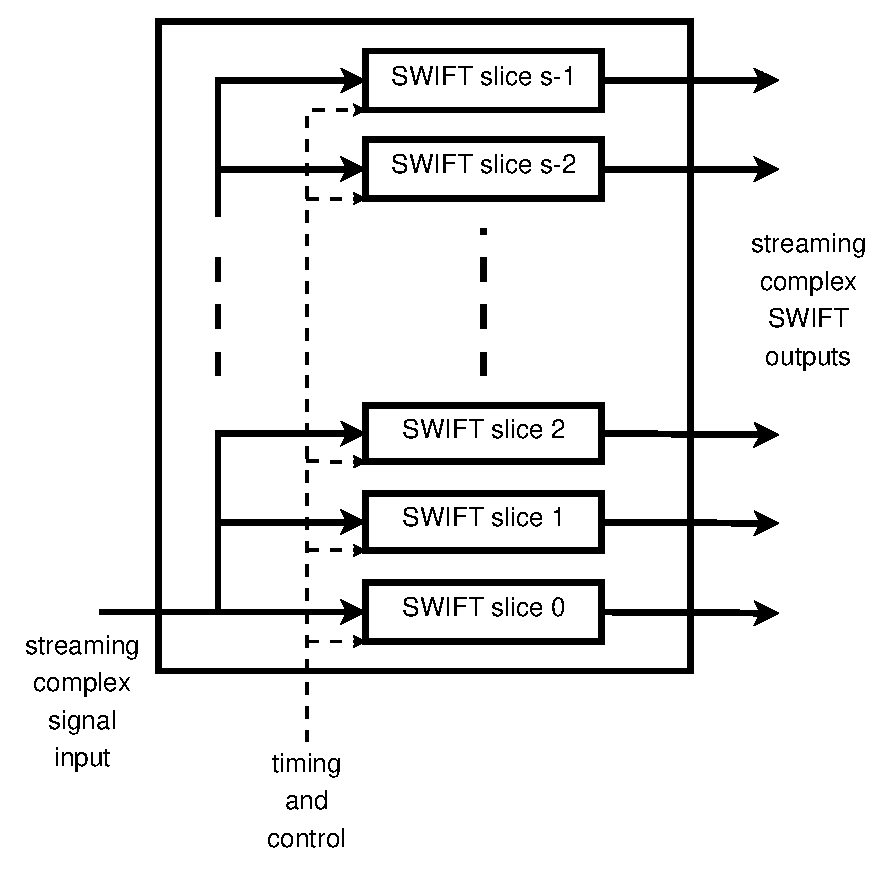
\includegraphics[width=\columnwidth]{Figures/fig_SWIFT_computation.eps}
\caption{Internal organization of SWIFT computation block}
\label{fig:SWIFT_slices}
\end{figure}



\begin{figure*}
\centering
\begin{tikztimingtable}
  	sample clock  	& 9.5L 3{9.5C} 9.5L \\
  	SWIFT clock   	& 95{0.5C}\\
  	sample  		& [timing/text format={\large}]9.5D{x[n-1]} N(S1) {} 19D{x[n]} {} 19D{x[n+1]}\\
 	\textbf{Adder} \\
  	FPADD out  		& [timing/text format={\large}]16.5D{$X_{n-1}(\omega_x)$} N(S2) {} N(FA1) 19D{$X_n(\omega_x)$} {} 12D{$X_{n+1}(\omega_x)$} \\
    \textbf{Mutliplier} \\
   	FPMUL out  		& [timing/text format={\large}]21.5D{$Dmul_{n-1}(\omega_x)$} {} N(FM1) 19D{$Dmul_n(\omega_x)$} {} 7D{} \\
    FPADD out  		& [timing/text format={\large}]28.5D{$Dadd_{n-1}(\omega_x)$} {} N(FA2) 19D{$Daddr_n(\omega_x)$} {} D{} \\ \\ 	
	\extracode
  	\tablerules
	\begin{pgfonlayer}{background}
    	\vertlines [help lines] {9.5,16.5,21.5,28.5};
        \node [anchor = mid ] at (13,-5){\small $cyc_{fa}$};
        \draw [<->] (9.5,-6) -- (16.5,-6);
        \node [anchor = mid ] at (19,-9){\small $cyc_{fm}$};
        \draw [<->] (16.5,-10) -- (21.5,-10);
        \node [anchor = mid] at (25,-15){\small $cyc_{fa}$};
        \draw [<->] (21.5,-16) -- (28.5,-16);
  	\end{pgfonlayer}
\end{tikztimingtable}
\caption{SWIFT slice timing waveform with time sharing}
\label{fig:SWIFT_slice_time_share_waveform}
\end{figure*}


required as well as  as shown in Figure \ref{fig:M_swift_slices}

\begin{figure}[tbp]
\centering
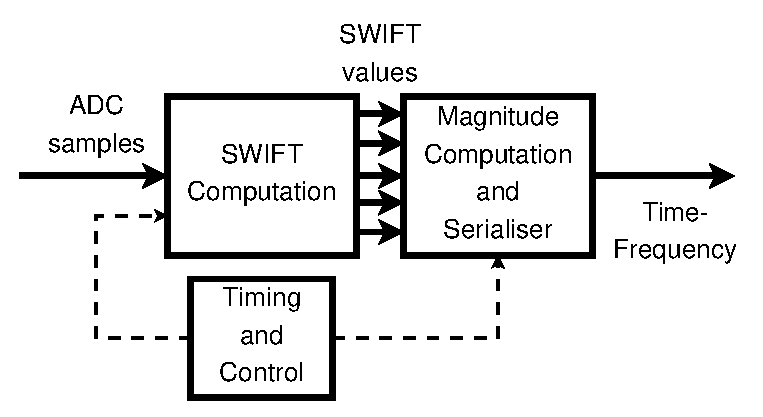
\includegraphics[width=\columnwidth]{Figures/fig_FPGA_system_diagram.eps}
\caption{System diagram of an FPGA implementation of the SWIFT algorithm}
\label{fig:FPGA_system_design}
\end{figure}


\section{Implementation Results and Comparison}
\label{Sec:Results}

The algorithm is implemented using Verilog and the target device chosen in an Intel/Altera Stratix IV EP4SGX230KF40C2ES. 

\begin{table}[!h]
\caption{FPGA implementation comparison}
\centering
\begin{tabular}{
	|P{0.25\columnwidth}
    |P{0.12\columnwidth}
    |P{0.12\columnwidth}
    |P{0.12\columnwidth}
    |P{0.12\columnwidth}|}
\hline
	Resource Utilization & Proposed design & M'jee 2015 & Zhou 2013 & Chandra 2013\\ \hline
	Resolution & not dependent on sample rate &\multicolumn{3}{P{0.36\columnwidth}|}{dependent on sample rate} \\ \hline
	Frequency bins & 570 & 64 & 1024 & 8\\ \hline
	Algorithm & SWIFT & 8-parallel Radix-2 FFT & Radix-2 FFT & Sliding Window DFT\\ \hline
	Device\ Used & Altera Stratix IV & Xilinx Virtex 5 & Altera Cyclone II & Stratix II \\ \hline
	Slice\ Registers & 39739 & 3082 & 372 & 1755\\ \hline
	Slice\ LUTs & 57501 & 12645 & 662 & 2409\\ \hline
	DSP\ slices\ uses & 328 & 48 & 8 & 128\\ \hline
	Memory\ kbits & 368 & Data\ unavailable & 82 & 5\\ \hline
	Clock\ Frequency\ (MHz) & 192 & 30 & 100 & Data unavailable\\ \hline
	Latency\ (ns) & $\sim$ 250 & Data\ unavailable & $\sim$ 62950 & Data unavailable\\ \hline
\end{tabular}
\label{table:FPGA_implementation_comparison}
\end{table}
\section{Conclusion}
\label{Sec:Conclusion}

The conclusion goes here.

% conference papers do not normally have an appendix

% use section* for acknowledgment
\section*{Acknowledgment}

The authors would like to thank...

% trigger a \newpage just before the given reference
% number - used to balance the columns on the last page
% adjust value as needed - may need to be readjusted if
% the document is modified later
%\IEEEtriggeratref{8}
% The "triggered" command can be changed if desired:
%\IEEEtriggercmd{\enlargethispage{-5in}}

% references section
\bibliographystyle{IEEEconf}
\bibliography{IEEEabrv,swift}



% that's all folks
\end{document}
